\documentclass[a4paper,fontsize=12pt,headsepline]{scrartcl}

\usepackage{changes}
% Defines
% \added[id=<author’s id>,remark=<remark>]{<new text>}
% \deleted[id=<author’s id>,remark=<remark>]{<old text>}
% \replaced[id=<author’s id>,remark=<remark>]{<new text>}{<old text>}

% \usepackage{soul}
% \newcommand{\fixme}[1]{\hl{#1}}
\newcommand{\fixme}[1]{\textsl{\textcolor{Orange}{fixme: #1}}}

\usepackage{graphicx}
%\usepackage[usenames]{color}

\usepackage[english]{babel}  
\usepackage[automark]{scrlayer-scrpage}
\usepackage{setspace}

\usepackage{float}
\usepackage{subcaption}  %%% newer version that can be used instead of subfigure
\usepackage[section]{placeins}

\usepackage{geometry}
\usepackage{url}


\usepackage{texshade} % MSA prints
\usepackage[]{amsmath} % Amsmath - Mathematik Basispaket
\usepackage{amssymb}


\usepackage{multirow}
\usepackage{array}


%%%%%%%%%% bibliography %%%%%%%%%%%%%%%%%%%%%%%%%%%%%%%
\usepackage[authoryear, sort, square]{natbib}
\bibliographystyle{cell}
%\usepackage[%
%	square,	% for square brackets;
%	comma,	% to use commas as separaters;
%	numbers,	% for numerical citations;
%	sort,		% orders multiple citations into the sequence in which they appear in the list of references;
%	sort&compress,    % as sort but in addition multiple numerical citations
%]{natbib}

%spaces between single entries
%\setlength{\bibsep}{3pt}
%%%%%%%%%%%%%%%%%%%%%%%%%%%%%%%%%%%%%%%%%%%%%%%%%%%%%


%\usepackage{subfig} % Layout wird weiter unten festgelegt !
%\usepackage{subfigure} % Layout wird weiter unten festgelegt !
% Aussehen der Captions fuer subfigures (subfig-Paket)
\usepackage[english,intoc]{nomencl}
%\usepackage{url} % Setzen von URLs. In Verbindung mit hyperref sind diese auch aktive Links.
\usepackage{ae} %erkennt umlaute
% sz
%\usepackage[latin1]{inputenc} 
\usepackage[utf8]{inputenc}

%\usepackage{caption}
\usepackage[font={sf,bf,small},textfont=md,textfont=md]{caption} 

% Aussehen der Captions
\captionsetup{
	margin = 5pt,
	font={sf,bf,small},
	textfont = {md,small},
	format = default, %singlespace% oder 'hang'
	indention = 0em,  % Einruecken der Beschriftung
	%labelsep = colon, %period, space, quad, newline
	%justification = RaggedRight, % justified, centering
	singlelinecheck = true, % false (true=bei einer Zeile immer zentrieren)
	position = bottom %top
}
%%% Bugfix Workaround
\DeclareCaptionOption{parskip}[]{}
\DeclareCaptionOption{parindent}[]{}
%\DeclareCaptionLabelFormat{andtable}{#1~#2 \& \tablename~\thetable}

% Aussehen der Captions fuer subfigures (subfig-Paket)
%\captionsetup[subfloat]{%
%   margin = 10pt,
%   font = {small,rm},
%   labelfont = {small,bf},
%   format = default, % oder 'hang'
%   indention = 0em,  % Einruecken der Beschriftung
%   labelsep = space, %period, space, quad, newline
%   justification = RaggedRight, % justified, centering
%   singlelinecheck = true, % false (true=bei einer Zeile immer zentrieren)
%   position = bottom, %top
%   labelformat = parens % simple, empty % Wie die Bezeichnung gesetzt wird
% }
%\setlength{\tabcolsep}{4pt} %distance between columns
%\renewcommand{\arraystretch}{0.75} %distance between rows in tables

\usepackage{setspace}


%\renewcommand{\baselinestretch}{1.5}%line spacing
%more figures allowed per page
\renewcommand\floatpagefraction{1}
\renewcommand\topfraction{1}
\renewcommand\bottomfraction{1}
\renewcommand\textfraction{0}   
\setcounter{totalnumber}{50}
\setcounter{topnumber}{50}
\setcounter{bottomnumber}{50}

%index
\usepackage{makeidx}
\makeindex


\newcommand{\nom}[2]{#1 \ \dotfill \ #2 \\}

%\usepackage{fancyhdr}
%\pagestyle{fancy}

%%%%%%%%%%%%%%%%% Page layout %%%%%%%%%%%%%%%%%%%%%%%%%%%

%\addtolength{\textheight}{3cm}
%\voffset-0.5cm
%\hoffset-1cm
%\addtolength{\textwidth}{2cm}


\geometry{a4paper, top=25mm, left=25mm, right=25mm, bottom=25mm,
	headsep=10mm, footskip=12mm}


%%%%%%%%%%%%%%%% Figure Path %%%%%%%%%%%%%%%%%%%%%%

%\usepackage{standalone}
%\standaloneconfig{mode=buildnew}
\graphicspath{{./figures/}}

\setlength{\parindent}{0pt} 

\begin{document}
	
	\setcounter{page}{0}\pagenumbering{Roman}
	%%%%%%%%%%%%%%%%%%%% Title, Table of Contents etc. %%%%%%%%%%%%%%%%%%%%%%%

\begin{titlepage}
	\centering
	{\normalsize Ruprecht-Karls-Universität Heidelberg \par}
	\vspace{0.25cm}
	{\normalsize Fakultät für Biowissenschaften \par}
	\vspace{0.25cm}
	{\normalsize Masterstudiengang Molekulare Biotechnologie \par}
	\vspace{3.5cm}
	{\LARGE \bfseries Systematic Expression Profiling of Chronic Lymphatic Leukemia Transcriptomes \par}
	\vspace{5cm}
	{\normalsize Masterarbeit \par}
	\vspace{4cm}
	{\normalsize\textbf{ Von Almut Lütge} \par}
	\vspace{0.25cm}
	{\normalsize\textbf{Aus Hildesheim} \par}
	\vspace{0.5cm}
	{\normalsize\textbf{Abgabetermin Dezember 2017}}
\end{titlepage}


\cleardoublepage

\begin{titlepage}

Die vorliegende Masterarbeit wurde am Deutschen Krebsforschungszentrum Heidelberg in der Abteilung für Computational Oncology in der Zeit von 08/06/2017 bis 08/12/2017 angefertigt.\par
\vspace{2.5cm}
Gutachter der Arbeit: \hspace*{12mm}	 Dr. Matthias Schlesner\par
					\hspace*{54mm}	Computational Oncology\par
					\hspace*{54mm}	Deutsches Krebsforschungszentrum Heidelberg\par
\vspace{1cm}
Zweitgutachter der Arbeit: \noindent\hspace*{3mm}	
Dr. Wolfgang Huber\par
\noindent\hspace*{56mm}Structural and Computational Biology\par
\noindent\hspace*{56mm}European Molecular Biology Laboratory \par
\vspace{2.5cm}
\hrule
\vspace{1.5cm}
Ich erkläre hiermit ehrenwörtlich, dass:
\begin{enumerate}
\item ich die vorliegende Masterarbeit selbständig unter Anleitung verfasst und keine anderen als die angegebenen Quellen und Hilfsmittel benutzt habe;
\item die Übernahme wörtlicher Zitate aus der Literatur/Internet sowie die Verwendung der Gedanken anderer Autoren an den entsprechenden Stellen innerhalb der Arbeit gekennzeichnet wurde;
\item ich meine Masterarbeit bei keiner anderen Prüfung vorgelegt habe.
\end{enumerate}
\vspace{0.25cm}
Ich bin mir bewusst, dass eine falsche Erklärung rechtliche Folgen haben wird. \par

\vspace{3.5cm}


Ort, Datum \hspace*{40mm}			Unterschrift\par


\end{titlepage}
\cleardoublepage
\onehalfspacing

\section*{Acknowledgements}

First of all, I want to thank Dr.~Junyan Lu and Dr.~Wolfgang Huber, who supervised this work with all their expertise and inspiring comments and feedback, but also invested a lot of time and patience to support me. I also want to thank for the chance to work on this project and even more the encouragement to learn so many new things and actively participate in all the exciting conferences, courses and retreats.\\
I want to thank Dr.~Matthias Schlesner and Dr.~Thorsten Zenz for their feedback and additional expertise. It was a real support. 
Many thanks to all members of the Huber group for the wonderful time, the support and all the chats at lunch or coffee breaks. I really enjoyed working with them. \\
My special thanks are to my twinsister Mechthild for her graceful support in every situation as well as to my sisters Barbara, Rosa and my parents for always being my backup.   


	\cleardoublepage
	
	\onehalfspacing	


%--------------------------------------------------0
\section*{Outline} 
%--------------------------------------------------0
%\subsection{Mixed epistatsis between Trisomy12 and IGHV status in Chronic Lymphocytic Leukemia} 

\textbf{Claim 1: Genomic variation in CLL is reflected on gene expression}: \\
    IGHV status and Trisomy12 are main drivers of gene expression variability. In line with this, expression of the 150 most variable genes is regulated by low-, intermediate and high programmed methylation groups. Other known variants show distinct expression profiles as TP53, SF3B1, Del11q22.3, Notch1 and Del13q14. In total 7 of 13 variants showed distinct expression  signatures. Expression of Marker genes ZAP70 and CD38 is up-regulated in U-CLL.\\
    \\
    \textit{Questions to solve:}\\
    1.How do we define distinct? All variants result in significantly differentially expressed genes using Deseq2. They vary in the number of significant genes (see figure \ref {fig:data_overview}) and how good they cluster on the expression of their differentially expressed genes. What is the best way to formalize this? Can we use the associations (t-test) of the variants and principal components of their significant genes (see figure \ref {fig:distinct_genes})
    2.Should we include an extra figure for the methylation groups? I already included the t-sne in figure 2, but I think it is a remarkable finding. Expression of the most variable genes are clearly associated to them and we can explain it by the expression of some multi-regulatory transcription factors (that have been proposed by Oakes et al.)
\\
    \\
    \\
\textbf{Claim 2: IGHV status and Trisomy12 interact (in an epistatic way) determining gene expression}: \\
     Sample with hypermutated IGHV and trisomy12 unravel gene cluster of different ways of epistatic interaction, so called mixed epistasis. We find sets of genes, that are affected by buffering, suppression, masking and inversion. These cluster represent..?  Drug sensitivity data (and prognosis?) support this evidence of epistatic interaction. \\
     \\
     \textit{Questions to solve:}\\
     %4. Test all other variants for epistatic effects -- to show that tri12 \& IGHV are ``special''\\
     4. Which of the other data sets can we use to support our model of epistasis? To what degree do we find epistasis in Mek/Erk inhibitors? Do we find evidence of epistasis in prognosis/metabolic data?
    \\
   

\begin{figure}
  \centering
  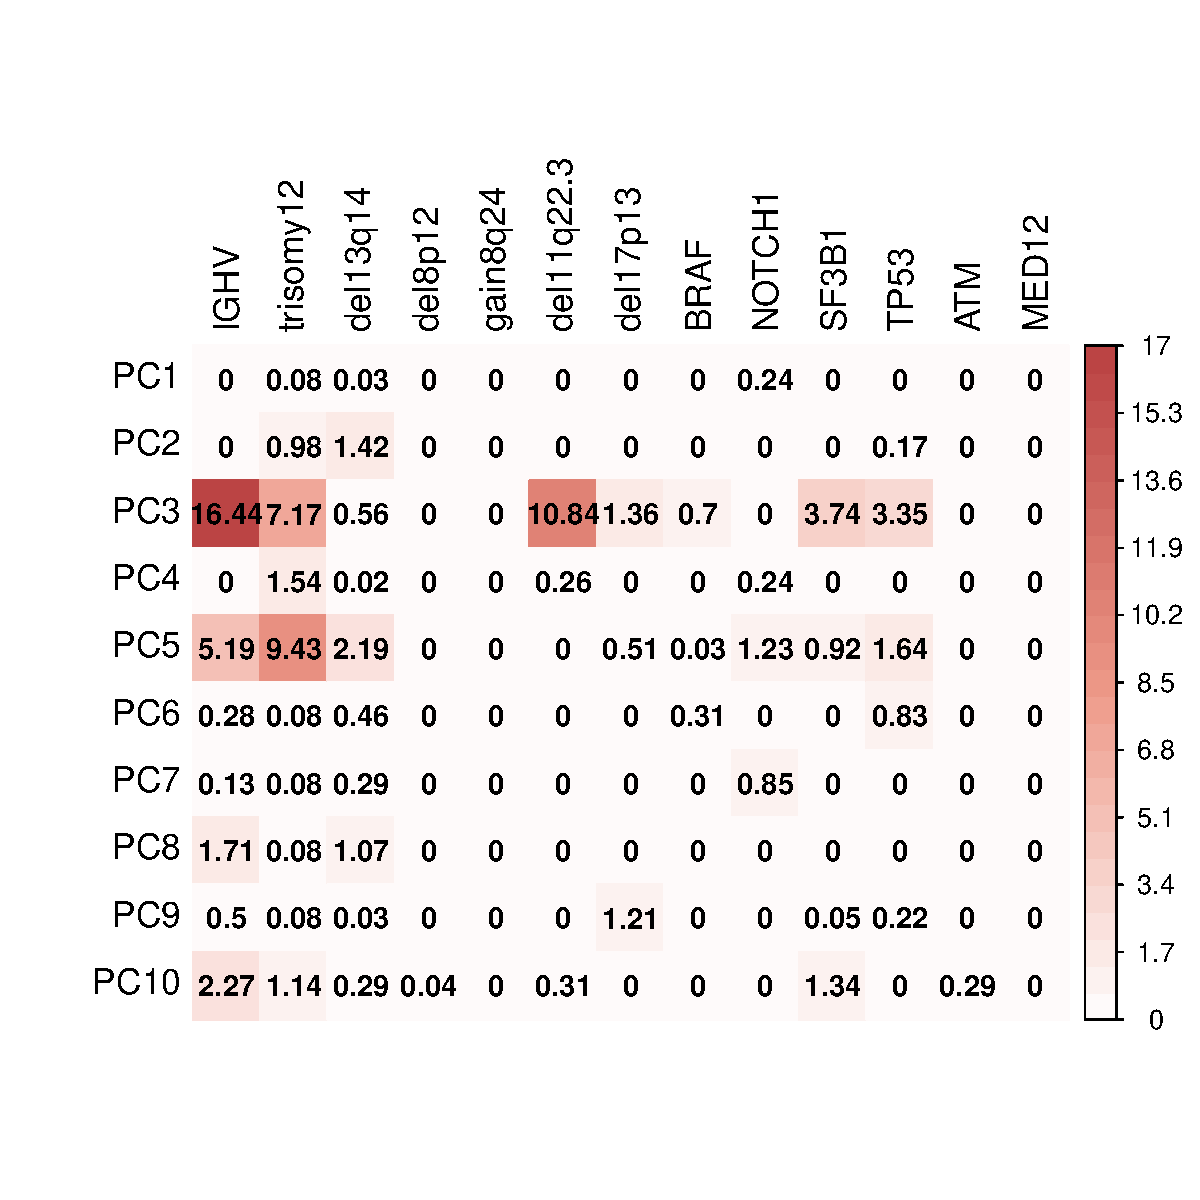
\includegraphics[width=\columnwidth]{figures/pca_variant_specific_genes.pdf}
  \caption{\textbf{Associations of variants and principal components in differentially expressed genes:} -$\log_{10}$(p.adjust) of t-test for associations between variants and the principal components within gene expression of significant ( $\text{p}_\text{adj} < 0.01$, $\log_2$fold change $>2$) results from differential expression analysis. In total 7 of 13 variants show significant associations to at least one of the first principal components describing the variance within gene expression based on results from differential expression analysis. \fixme{This analysis and figure has some merit, but it's too abstract / too complex for a main figure. I think it'd better to just state the number of DE genes (at a fixed FDR, say 10\%) for each mutation. Also, I have an idea for a PCA plot which we can discuss on the phone. Basically: choose top 2000 (or so) genes (or the union of the above?), for each mutation compute the difference of means between groups of samples with and without, which results in 13 vectors of length 2000, then display these 13 points in a 2D PCA.}}
  \label{fig:distinct_genes}
\end{figure} 


\cleardoublepage

\onehalfspacing
\setcounter{page}{0}\pagenumbering{arabic}
\pagestyle{headings}


\end{document}